\section{Vision}
% Sources:
% https://0xbrainjar.medium.com/our-vision-for-composable-finance-ab6518d7e617

A natural evolution in a cross-chain world entails developers and users interacting seamlessly with protocols, regardless of where their assets live. That is why our core mission at Composable Finance (Composable) \cite{ComposableFinance}, is to build a fully interoperable future, capable of offering developers and end-users a seamless experience and utility.
%
Through simplifying and unifying decentralized finance (DeFi) \cite{DecentralizedEthereum.org} with new interoperability standards we are accelerating DeFi into the mainstream. We are crafting a transparant, interoperable future for DeFi 2.0 and Web3.

Similar to how Port Control Protocol \cite{PortWikipedia} became an essential piece of the networking layer for the Internet, Composable's vision is to become the entryway and networking fabric for blockchain networks. It is Composable's mission to service all interactions, transfers, and communication cross-ecosystem.
%
Our vision of hyper liquidity and composability abstract the underlying technology into a single interface, unlocking the potential for new primitives to be developed at an unprecedented pace. Protocol-to-protocol interactions will become possible across ecosystems.

The DeFi space has resorted to sharded blockchains for increased scalability \cite{WhyProperties,WhatCoinDesk}. Examples are Ethereum 2.0 \cite{TheEthereum.org}, Polkadot \cite{Polkadot:Platform}, and NEAR \cite{NEARWorld}. The result, however, is that even though the vision of ETH 2.0 is already upon us, instead of just blockchains being sharded, applications are being sharded as well. SushiSwap \cite{IntroductionSushi}, for example, is deployed on multiple Ethereum Virtual Machine (EVM) \cite{EthereumEthereum.org} compatible chains, Layer-2-like (L2) rollups \cite{LayerEthereum.org}, and Parachains \cite{WhatAlexandria}, and the expansion of these applications to other ecosystems is very likely. Thus, while moving assets intra-ecosystem is becoming more intuitive, with several applications segregated within a specific ecosystem, managing assets inter-ecosystem is not \cite{0xbrainjarOurMedium}.

Therefore, Composable is focused on a cross-chain, cross-layer liquidity layer for sharded applications. Composable takes this notion a step further by also realizing that between each ecosystem, there is a sharding of functionality itself; for instance, most ecosystems have their own lending protocols. Our vision is thus to abstract away inter-ecosystem decision making and maximize users' and developers' outcomes based on their unique goals.

To accomplish this function, we are creating a communication protocol, utilizing our parachain as a finality layer, that will connect L2s to the Polkadot and Kusama ecosystem, and the Cosmos Ecosystem \cite{Cosmos:Blockchains} through the Inter-Blockchain Communication protocol (IBC) \cite{Inter-BlockchainCommunication} to the Polkadot and Kusama ecosystem.
%
We will then include other ecosystems, such as Algorand \cite{AlgorandAlgorand}, Solana \cite{ScalableScale}, and more.

We are embarking on a vast and growing opportunity in architecting and building infrastructure that allow developers to deploy applications capable of interoperating across layers and chains autonomously.
%
We believe that the applications of such a stack are the catalyst for the next DeFi revolution.

\begin{figure}
    \centering
    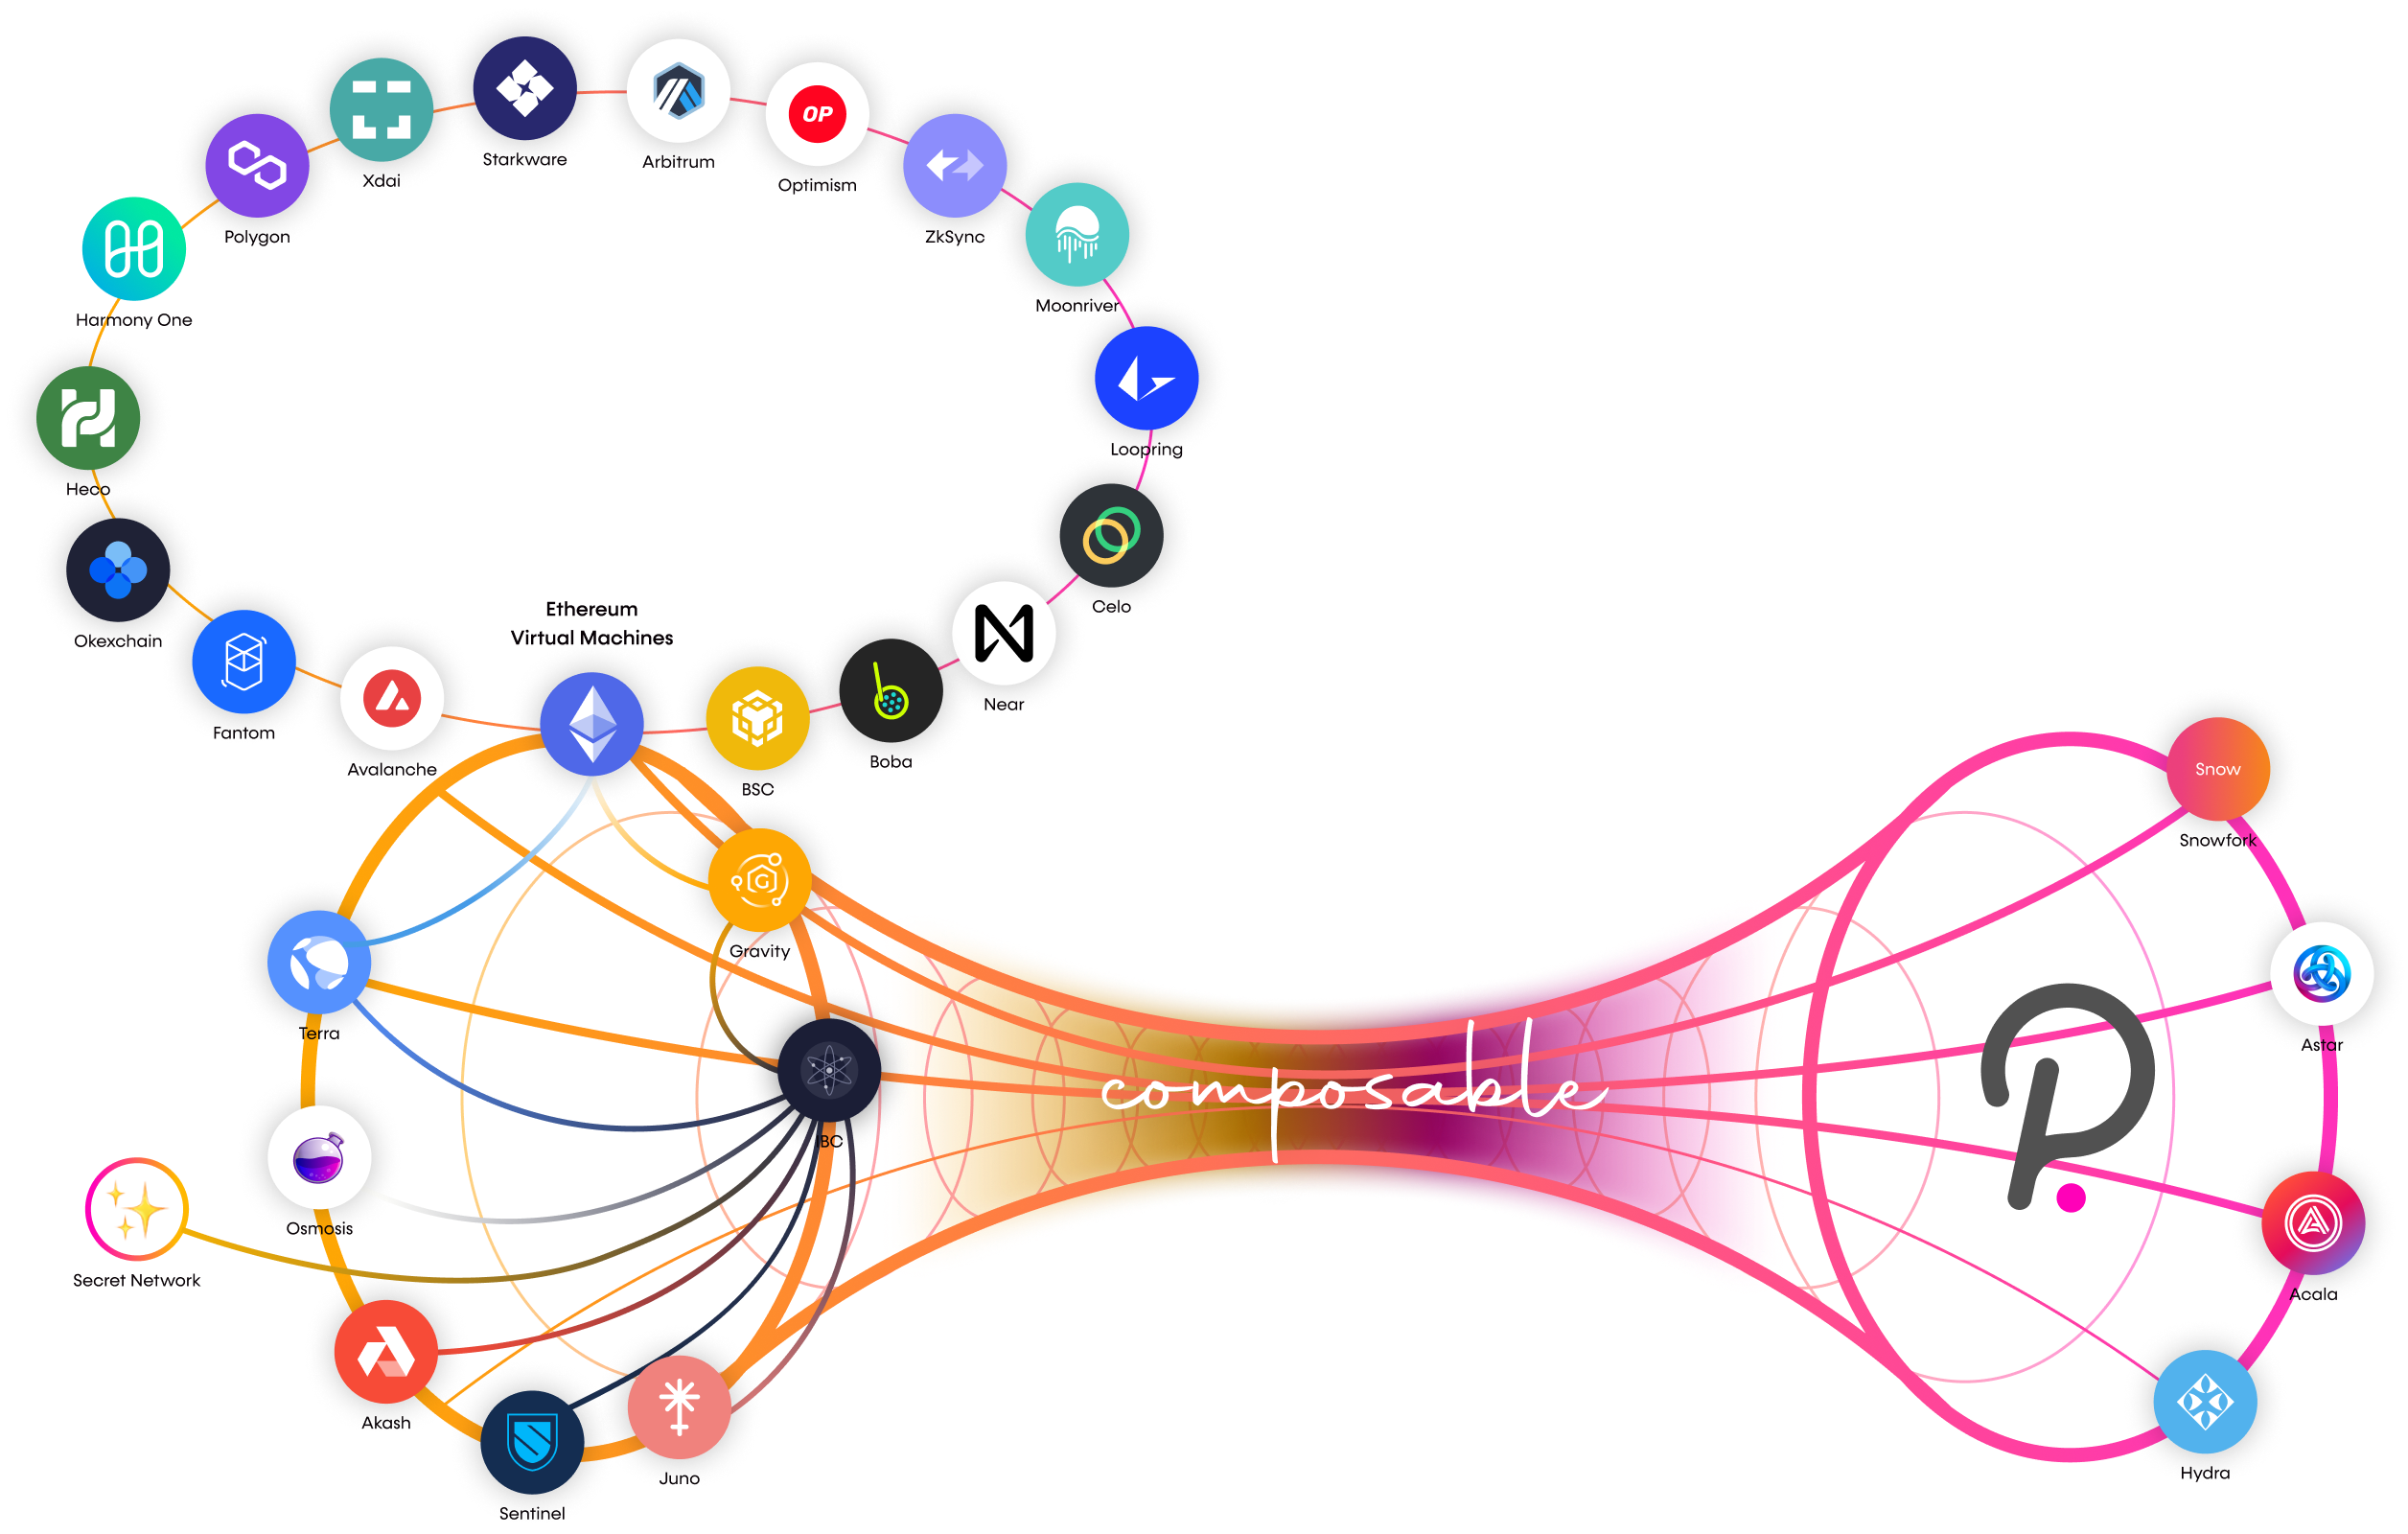
\includegraphics[scale=0.28]{images/parachain.png}
\end{figure}
